% 48-21(48쪽) — $y=\log_a x$, $y=\log_b x$ 와 두 직선 $y=1$, $y=2$ 의 교점 A·B·C·D(원문 「오른쪽 그림」). 스캔 화질이 낮아 TikZ 로 다시 그림.
% 라벨은 원문에 있는 것만 — 두 곡선 이름, 점 A·B·C·D, $y$축 눈금 1·2 와 두 직선 이름, 원점 O.
% 밑 $a$, $b$ 는 원문처럼 $x$축 눈금 없이 그려 $\seg{CD}$(답)가 그림에서 읽히지 않게 한다.
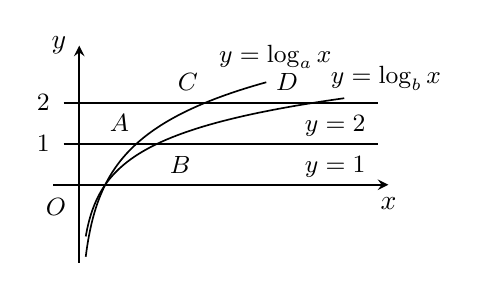
\begin{tikzpicture}[line width=0.6pt, x=0.33cm, y=0.52cm, >=stealth]
  \draw[->, line width=0.7pt] (-1.0,0) -- (11.9,0) node[below=1pt] {$x$};
  \draw[->, line width=0.7pt] (0,-1.9) -- (0,3.4) node[left=1pt] {$y$};
  \draw[line width=0.5pt] (-0.6,1) -- (11.5,1);
  \draw[line width=0.5pt] (-0.6,2) -- (11.5,2);
  \draw[domain=0.25:7.2, samples=180, smooth] plot (\x, {ln(\x)/ln(2.2)});
  \draw[domain=0.25:10.2, samples=180, smooth] plot (\x, {ln(\x)/ln(3)});
  \node[font=\small, anchor=south east] at (2.30,1.06) {$\pt{A}$};
  \node[font=\small, anchor=north west] at (3.10,0.94) {$\pt{B}$};
  \node[font=\small, anchor=south east] at (4.95,2.06) {$\pt{C}$};
  \node[font=\small, anchor=south east] at (8.80,2.06) {$\pt{D}$};
  \node[font=\small, anchor=east] at (-0.75,1.0) {$1$};
  \node[font=\small, anchor=east] at (-0.75,2.0) {$2$};
  \node[font=\small, anchor=north east] at (-0.12,-0.10) {$\pt{O}$};
  \node[font=\small, anchor=west] at (5.0,3.12) {$y=\log_a x$};
  \node[font=\small, anchor=west] at (9.3,2.60) {$y=\log_b x$};
  \node[font=\small, anchor=north east] at (11.4,1.94) {$y=2$};
  \node[font=\small, anchor=north east] at (11.4,0.94) {$y=1$};
\end{tikzpicture}
